%%%%%%%%%%%%%%%%%%%%%%%%%%% asme2ej.tex %%%%%%%%%%%%%%%%%%%%%%%%%%%%%%%
% Template for producing ASME-format journal articles using LaTeX    %
% Written by   Harry H. Cheng, Professor and Director                %
%              Integration Engineering Laboratory                    %
%              Department of Mechanical and Aeronautical Engineering %
%              University of California                              %
%              Davis, CA 95616                                       %
%              Tel: (530) 752-5020 (office)                          %
%                   (530) 752-1028 (lab)                             %
%              Fax: (530) 752-4158                                   %
%              Email: hhcheng@ucdavis.edu                            %
%              WWW:   http://iel.ucdavis.edu/people/cheng.html       %
%              May 7, 1994                                           %
% Modified: February 16, 2001 by Harry H. Cheng                      %
% Modified: January  01, 2003 by Geoffrey R. Shiflett                %
% Use at your own risk, send complaints to /dev/null                 %
%%%%%%%%%%%%%%%%%%%%%%%%%%%%%%%%%%%%%%%%%%%%%%%%%%%%%%%%%%%%%%%%%%%%%%

%%% use twocolumn and 10pt options with the asme2ej format
\documentclass[twocolumn,10pt]{asme2ej}

\usepackage{graphicx} %% for loading jpg figures
\usepackage{amsmath, amssymb}
\usepackage{bm}
\usepackage{array}
\usepackage{caption}

% Useful definitions
\DeclareMathOperator*{\argmin}{argmin}
\DeclareMathOperator*{\argmax}{argmax}

%% The class has several options
%  onecolumn/twocolumn - format for one or two columns per page
%  10pt/11pt/12pt - use 10, 11, or 12 point font
%  oneside/twoside - format for oneside/twosided printing
%  final/draft - format for final/draft copy
%  cleanfoot - take out copyright info in footer leave page number
%  cleanhead - take out the conference banner on the title page
%  titlepage/notitlepage - put in titlepage or leave out titlepage
%  
%% The default is oneside, onecolumn, 10pt, final


\title{A unified framework for computer model calibration and engineering design}

%\author{Blinded version
%	\affiliation{
%		for review}
%}	

%%% first author
\author{Carl Ehrett
    \affiliation{
	Research Associate\\
	Watt Family Innovation Center\\
	Clemson University\\
	Clemson, South Carolina 29631\\
    Email: cehrett@clemson.edu
    }	
}
%%% second author
%%% remove the following entry for single author papers
%%% add more entries for additional authors
\author{D. Andrew Brown\thanks{Corresponding author.} 
    \affiliation{Associate Professor\\
    School of Mathematical and \\Statistical Sciences\\
	Clemson University\\
	Clemson, South Carolina 29631\\
	Email: ab7@clemson.edu
	}	
}
%%% third author
%%% remove the following entry for single author papers
%%% add more entries for additional authors
\author{Christopher Kitchens
   \affiliation{Associate Professor\\
       Department of Chemical\\and Biomolecular Engineering\\
       Clemson University\\
       Clemson, South Carolina 29631\\
       Email: ckitche@clemson.edu
   }}
\author{Sez Atamturktur
	\affiliation{Professor\\
		Department of Architectural Engineering\\
		The Pennsylvania State University\\
		University Park, Pennsylvania 16802\\
		Email: sez@psu.edu
}}
\author{Leslie Xu
	\affiliation{
		Graduate Research Assistant\\
		Department of Architectural Engineering\\
		The Pennsylvania State University\\
		University Park, Pennsylvania 16802\\
		Email: xkx5055@psu.edu
}}
\author{Roland Platz
	\affiliation{
		TODO TITLE\\
		TODO AFFILIATION\\
		Email: rxp5110@psu.edu
}}

\begin{document}
	
\maketitle    

%%%%%%%%%%%%%%%%%%%%%%%%%%%%%%%%%%%%%%%%%%%%%%%%%%%%%%%%%%%%%%%%%%%%%%
\begin{abstract}
	{\it 
		Calibration of computer models and the use of those models for design are two activities that are traditionally carried out separately.
		%
		This paper generalizes existing Bayesian inverse analysis approaches for computer model calibration to present a methodology combining calibration and design under a unified Bayesian framework.
		%
		This provides a computationally efficient means to undertake both tasks in a way that quantifies all relevant sources of uncertainty.
		%
		Specifically, compared with the traditional approach of design using parameter estimates made during previously completed model calibration, this generalized framework inherently includes uncertainty from the calibration process in the design procedure.
		%
		We demonstrate our approach for simultaneous calibration and design in a dynamic vibration system.
		%
		We also demonstrate how, when adaptive sampling of the phenomenon of interest is possible, the proposed framework may select new sampling locations using both the available real observations and the computer model.
		%
		This is especially useful when the model is misspecified in failing to reflect that the parameter to be calibrated is functionally dependent upon the design inputs that are to be optimized.
		%
	}
\end{abstract}

%%%%%%%%%%%%%%%%%%%%%%%%%%%%%%%%%%%%%%%%%%%%%%%%%%%%%%%%%%%%%%%%%%%%%%
\begin{nomenclature}
	\entry{$\beta$}{Inverse correlation length for Gaussian process input}
	\entry{$\delta(\cdot)$}{Discrepancy between model and true system}
	\entry{$\epsilon_c$}{Measurement error}
	\entry{$\epsilon_d$}{Discrepancy between optimal system output and $\boldsymbol y_t$}
	\entry{$\eta(\cdot)$}{Computer model of the system of interest}
	\entry{$\zeta$}{Damping ratio of a dynamic vibration system}
	\entry{$\boldsymbol\eta$}{Vector of outputs of $\eta(\cdot)$}
	\entry{$\boldsymbol\theta_c$}{True value of parameter to be calibrated}
	\entry{$\boldsymbol\theta_d$}{Optimal design input}
	\entry{$\lambda$}{Marginal precision of Gaussian process}
	\entry{$\rho$}{Reparameterization of $\beta$}
	\entry{$\sigma^2_c$}{Variance of $\epsilon_c$}
	\entry{$\sigma^2_d$}{Variance of $\epsilon_d$}
	\entry{$\boldsymbol\phi_\delta$}{Hyperparameters of Gaussian process model of $\delta(\cdot)$}
	\entry{$\boldsymbol\phi_\eta$}{Hyperparameters of Gaussian process surrogate for $\eta(\cdot)$}
	\entry{$\mathcal D$}{($\boldsymbol\eta^T,\mathbf y^T)^T$ for some observations $\mathbf y$}
	\entry{$C_\eta(\cdot)$}{Covariance of Gaussian process emulator of $\eta$}
	\entry{$C_\delta(\cdot)$}{Covariance of Gaussian process model of $\delta$}
	\entry{$k$}{Elastic modulus of leaf spring}
	\entry{$f(\cdot)$}{The system of interest}
	\entry{$g$}{Gain of dynamic vibration system}
	\entry{$m$}{Mass of oscillator in dynamic vibration system}
	\entry{$m_\eta(\cdot)$}{Mean of Gaussian process emulator of $\eta$}
	\entry{$m_\delta(\cdot)$}{Mean of Gaussian process model of $\delta$}
	\entry{$T$}{Time period of one oscillation of a dynamic vibration system}
	\entry{$t_c$}{Value of calibration parameter used as input in $\eta(\cdot)$}
	\entry{$t_d$}{Value of design variable used as input in $\eta(\cdot)$}
	\entry{$\mathbf x$}{All model inputs in the operational domain of $f(\cdot)$}
	\entry{$\mathbf y_r$}{Vector of observations of the system of interest}
	\entry{$\mathbf y_s$}{Vector of outputs of the computer model of $f(\cdot)$}
	\entry{$\mathbf y_t$}{Vector of target outcomes for the system of interest}
	\entry{$\mathbf z$}{All known and/or controllable inputs of $f(\cdot)$}
\end{nomenclature}
%%%%%%%%%%%%%%%%%%%%%%%%%%%%%%%%%%%%%%%%%%%%%%%%%%%%%%%%%%%%%%%%%%%%%%%%%%%%%%

%\thanks{The authors gratefully acknowledge grant CMMI-1934438 from the National Science Foundation (NSF). CE was supported by fellowships through Department of Education GAANN grant P200A150310 and NSF NRT grant 1633608. DAB is also supported by NSF grants EEC-1744497 and OIA-1826715.}\hspace{.2cm}\\

%{\it Keywords: Gaussian processes, optimization, uncertainty quantification, computer model calibration, engineering design}  

\section{Introduction}\label{sec:introduction}

%
This paper connects two distinct areas of research concerning computer models of real phenomena.
%
One area is that of computer model calibration, where the goal is to find a posterior distribution on unknown, or imperfectly known, parameters by calibrating a computer model using real-world observations of the modeled phenomenon.
%
The second area is that of enlisting a computer model for design, using the model to find settings for controllable system inputs such that the resulting system output is optimized with respect to some design goal.
%
These two problems are structurally similar, both involving finding estimates or distributions of model inputs to achieve some desired effect on model outputs.
%
In the case of calibration, the desired effect is that the model outputs approximate reality, and in the case of design, the desired effect is that the model outputs approximate the optimal achievable outputs.
%
Since calibration and design are typically carried out separately, existing design techniques operate under the assumption that the model is an accurate approximation of the real system of interest.
%
In practice, models used for design typically are known or suspected to be biased representations of the phenomenon of interest, and often have inputs that require calibration.
%
The goal of the work described here is to provide a unified framework for calibration and design.
%
We refer to this new approach as DCTO, for dual calibration to target outcomes.
%
In addition to avoiding the idealization that the model used for design is unbiased, DCTO allows one to focus calibration efforts on regions of interest, prioritizing them over other areas of the model range.
%
For example, one may be more interested in calibrating the model to be accurate in the optimal region of some design variable $\boldsymbol \theta_d$ than elsewhere.
%
Having a combined framework for calibration and design is especially of interest when those two activities are non-trivially intertwined, as in the case when the value of the calibration parameters are functionally dependent upon the design settings.
%

%
Bayesian methods for computer model calibration are developed by Kennedy and O'Hagan \cite{Kennedy2001}.
%
Since their seminal paper, the methodology has seen numerous extensions and refinements (\cite{Higdon2004,Williams2006,Bayarri2007a,Bayarri2007b,Paulo2012,Brynjarsdottir2014}).
%
Henceforth, we refer to this approach to calibration as KOH.
%
Common to KOH approaches is the Bayesian framework in which one places a prior on the calibration parameters $\boldsymbol \theta_c$, often pairing it with a Gaussian process (GP) meta-model of the computer model of interest and a GP prior on the model discrepancy $\delta(\cdot)$, and using the available observations $y_r$ of the real system to find a posterior distribution $\boldsymbol\theta_c,\delta(\cdot)|y_r$.
%
Such an approach is notable for providing not merely a point estimate of the calibration parameter, but for providing a full posterior distribution quantifying remaining uncertainty about $\boldsymbol\theta_c$ and about $\delta(\cdot)$.
%

%
Herein, we leverage the KOH framework to find a posterior distribution, not only on unknown model parameters, but also on controllable design settings.
%
We achieve this via an approach called counterfactual Bayes.
%
In traditional model calibration, one uses Bayes' rule to discover a posterior distribution on calibration parameters using real observations, so that the observations are the source of the Bayesian learning.
%
In a design case, there are no relevant observations.
%
One wants to find design settings that induce the system to behave optimally, but one typically has not observed the system doing so, and therefore there seems to be no relevant source of Bayesian learning that could drive the use of Bayes' rule to discover a posterior distribution on optimal design settings.
%
The idea of counterfactual Bayes is to identify artificial observations, or target outcomes, $y_t$ such that the resulting likelihood is highest in the optimal design region --- i.e., target outcomes $y_t$ such that their occurrence is strong evidence that the design settings are optimal.
%
Hence, in addition to calibrating the unknown model parameters against experimental observations, one uses the KOH framework to also find a posterior distribution on design settings given the target outcomes --- and given the nature of $y_t$, this is \textit{de facto} a distribution on optimal design settings for the system.
%
The result retains the benefits of the Bayesian model calibration tools on which it is based, namely the quantification of remaining uncertainty regarding the optimal design settings.
%
And like KOH, DCTO is especially well-suited to problems that rely on black-box functions.
%

%
We may divide optimization approaches in such cases broadly into three camps \cite{Regis2004}.
%
Gradient-based approaches \cite{Nocedal2006} are of limited utility when dealing with black-box functions, where we cannot evaluate the objective function's derivative.
%
Approximation of the derivative requires additional function evaluations, rapidly inflating the computational cost when each evaluation involves significant expense.
%
Heuristic approaches \cite{Lee2007} such as evolutionary algorithms \cite{Branke2008,Deb2002,Kim2004}, particle swarm optimization \cite{Bonyadi2017,Mason2017}, and simulated annealing \cite{Robert2004} avoid the need to know or approximate derivatives, but often require prohibitively many function evaluations.
%
Furthermore, such methods, like gradient-based approaches, do not inherently provide quantification of remaining uncertainty about optimal design settings and the system outputs at those settings.
%
Methods exist for using heuristic approaches while accommodating and quantifying uncertainties \cite{Deb2006,Zhou2011b}, but these come at the cost of even further inflating the number of function evaluations required.
%
This problem can be mitigated by relying on a surrogate model, but the resulting uncertainty quantification is accomplished by separate methods that are layered on top of the independent heuristic approach.
%
On the other hand, our approach includes uncertainty quantification as an intrinsic aspect of the DCTO framework.
%

%
The third camp is the diverse collection of response surface methodologies (RSMs) \cite{Dean2017} used for optimization.
%
RSMs operate by fitting a predictive model to an existing set of model runs, to form a computationally inexpensive meta-model which is then used to explore the model output.
%
The concept of calibration to target outcomes that is built into DCTO is an example of an RSM, using GPs for its meta-model fit.
%
Other popular versions of RSMs include efficient global optimization (EGO) \cite{Jones1998,Brochu2010} and stepwise uncertainty reduction (SUR) \cite{Geman1996,Villemonteix2009,Chevalier2014,Picheny2015,MiguelHernandez-Lobato2016,Picheny2019,Binois2019}.
%
EGO and SUR are both designed to facilitate sequential sampling from the system of interest in a search for the global optimum.
%
They differ in their \textit{acquisition functions}, which determine the location of the next sampling location throughout the optimization process.
%
EGO finds the spot that maximizes the expected improvement \cite{Mockus1978,Jones1998}, whereas SUR's acquisition function seeks to reduce the volume of excursion sets below the current best known solutions \cite{Chevalier2014}.
%
Because they rely on sequential sampling, EGO and SUR are of limited utility when one is constrained to rely on a pre-existing set of observations, or in general when the observation locations cannot be chosen purely to suit the goal of optimization.
%
Furthermore, the acquisition functions employed by EGO and SUR attempt to balance exploitation (proposing a new sample location that optimizes system output) with exploration (proposing a location that promotes learning for subsequent rounds of sampling).
%
As a result, although these acquisition functions constitute distributions of sampling locations, by their nature they are not interpretable as distributions of the \textit{optimal} design settings for a given problem, and hence these distributions do not quantify uncertainty regarding the location of that optimum.
%
By contrast, our approach (understood as a pure-exploitation method) quantifies remaining uncertainty regarding the location of the system optimum.
%

%
An example of an RSM more closely resembling our approach to design is described by Olalotiti-Lawal and Datta-Gupta \cite{Olalotiti2018}.
%
Their approach defines a distribution which is designed to lie both on and near the Pareto front (PF) of the objective function and generates a posterior distribution which includes quantified uncertainties via Markov chain Monte Carlo (MCMC) \cite{Gelfand1990}.
%
However, their posterior distribution is designed by the authors and is not dictated by the model itself; as such, its interpretability is not entirely clear.
%
By contrast, our approach provides a posterior distribution based on the likelihood of the optimal design settings given the (hypothetical) observation of target outcomes $y_t$, and thus the uncertainty quantified by design using the KOH framework is model-driven and interpretable as uncertainty regarding the optimal values for the design inputs and the resulting system output.
%

%
The rest of the paper is organized as follows.
%
Section \ref{sec:dcto} describes the difficulties involved in extending KOH into a framework that incorporates both design and calibration, illustrating this by considering the failings of a na\"ive method for combining the two procedures, followed by a description of the proposed DCTO framework for extending KOH.
%
%Section \ref{sec:example} showcases the methodology using a synthetic example, demonstrating its thorough quantification of the relevant uncertainties.
%
Section \ref{sec:as} considers how DCTO may be useful in the case where sequential sampling is possible.
%
In particular, sequential sampling with DCTO is attractive when the calibration parameter is known or suspected to be functionally dependent upon the design settings.
%
We showcase the application of DCTO with sequential sampling using a synthetic example, comparing its results to that of a more traditional approach of design following calibration.
%
In Section \ref{sec:dvs} we apply DCTO to a dynamic vibration system, using a set of experimental observations simultaneously to calibrate a finite element model and to select optimal gain settings to minimize the system's damping ratio, and demonstrating DCTO's thorough quantification of the relevant uncertainties.
%
Section \ref{sec:conclusion} concludes with discussion of the results and thoughts about future directions.\footnote{
%
Note that KOH is usually conceived of as a means of calibrating a computer model with respect to a set of experimental observations.
%
However, the KOH framework, and by extension DCTO, are applicable more generally whenever one has access to both low-fidelity and high-fidelity sources of information and seeks to calibrate the former with respect to the latter.
%
This includes the case in which both the high-fidelity and low-fidelity sources of information are computer models (e.g. with different levels of computational expense).
%
For ease of exposition, we follow the common convention, and present DCTO in terms of calibrating a computer model using experimental observations.
%
Nonetheless, in some cases (such as in our discussion of sequential sampling in Section \ref{sec:as}), the methods discussed may apply more naturally in the context of employing two computer models of varying fidelity.
%
}
%

%
\section{Dual calibration to target outcomes}\label{sec:dcto}
%% Describe KOH model
%
The version of KOH considered here is that which finds a posterior distribution on a parameter of interest for calibration, $\boldsymbol\theta$, using a GP emulator with hyperparameters ${\boldsymbol\phi_\eta}$.
%
Similarly, one may also use a GP prior with hyperparameters $\boldsymbol\phi_\delta$ to model discrepancy between the computer model $\eta(\cdot)$ and the true function $f(\cdot)$ that it represents.
%
In the work described here, we employ stationary GPs with a Gaussian kernel covariance structure $C(\mathbf x,\mathbf x') = 1/\lambda \times \exp(-\beta(\mathbf x-\mathbf x')^2)$, so that ${\boldsymbol\phi_\eta} = \left[\beta,\ \lambda\right]$.
%
In our adaptation, $\boldsymbol\theta=(\boldsymbol\theta_c,\boldsymbol\theta_d)$ is partitioned into parameters $\boldsymbol\theta_c$ to be calibrated and inputs $\boldsymbol\theta_d$ to be optimized for design purposes.
%
Setting priors on $\boldsymbol\theta$ and on $\boldsymbol \phi_\delta$, we train the GP emulator on observations $\boldsymbol \eta$ and use MCMC to explore the distribution
\begin{equation} \label{eq:full_dist}
\pi(\boldsymbol \theta,{\boldsymbol\phi_\eta},\boldsymbol \phi_\delta|\mathcal D)
\propto \pi(\mathcal D | \boldsymbol \theta_,{\boldsymbol\phi_\eta}, \boldsymbol\phi_\delta) %\times \pi(\lambda_\eta) 
%\times \pi(\boldsymbol \rho^\eta) 
\times \pi(\boldsymbol\theta)
\times \pi(\boldsymbol\phi_\eta)
\times \pi(\boldsymbol\phi_\delta)
\end{equation}
%
where $\mathcal D = (\boldsymbol\eta^T,\ \mathbf y^T)^T$ for some observations $\mathbf y$.
%

%
In a computer calibration problem, $\mathbf y$ is a set of observations of the system modeled by $\eta()$.
%
When calibrating to target outcomes as in DCTO, by contrast, $y$ is a set of target outcomes representing the way that one wishes to induce the system to behave (rather than observations one has made of the system in reality).
%
When one wishes to perform design leveraging a simulation model that also requires traditional calibration, then, one might consider combining the two approaches by using Equation \eqref{eq:full_dist} with $\mathbf y= (\mathbf y_r^T,\ \mathbf y_t^T)^T$, an array containing both real observations $\mathbf y_r$ (for calibration) and target outcomes $\mathbf y_t$ (for design).
%
However, this approach will not work, both because the inputs to be calibrated are typically not the same as the design settings under researcher control, and also because for successful calibration one must train one's model on observations of reality rather than on unobserved target outcomes.
%

%
Hence, model calibration and system design must be separated.
%
An obvious choice here is to perform KOH calibration first, without involving any target outcomes, and then to use the calibrated model in order to perform CTO.
%
Under this approach, with observations $
\mathbf y_r$ of the system of interest, one would employ the model described in Equation \eqref{eq:full_dist} with $\boldsymbol \theta = \boldsymbol \theta_c$ (the parameters to be calibrated) and with $\mathcal D = \mathcal D_c = (\boldsymbol\eta^T, \mathbf y_r ^T)^T$.
%
The result would be a posterior distribution of $\boldsymbol \theta_c$ and of $\delta(\cdot)$, the systematic discrepancy between the computer model $\eta(\cdot,\cdot)$ and the true system $f(\cdot)$.
%
These can be used to produce estimates $\widehat{\boldsymbol\theta_c}$ and $\widehat\delta(\cdot)$ such that $f(\mathbf z)\approx\eta(\mathbf z,\widehat{\boldsymbol\theta_c})+\widehat\delta(\mathbf z)$ for all $\mathbf z$ in the domain of $f$.
%
The result is a calibrated model $\eta_c(\mathbf z)=\eta(\mathbf z,\widehat{\boldsymbol\theta_c})+\widehat\delta(\mathbf z)$ which can be used for design.
%

%
With $\eta_c$ in hand, one can partition $\mathbf z$ into $(\mathbf x,\boldsymbol\theta_d)$ where $\boldsymbol\theta_d$ is the set of inputs over which one wishes to optimize, and $\mathbf x$ are all other inputs in the operational domain, within which the calibrated model's predictions are reliable.
%
We can write $\eta_c(\mathbf z)$ as $\eta_c(\mathbf x,\boldsymbol\theta_d)$.
%
Then one can perform design again using Equation \eqref{eq:full_dist}, this time with $\boldsymbol\theta = \boldsymbol\theta_d$ and $\mathcal D = \mathcal D_t = (\boldsymbol\eta_c^T,\mathbf y_t^T)^T$ where $\boldsymbol\eta_c = \boldsymbol \eta+ \widehat{\boldsymbol \delta}= \boldsymbol \eta+ (\widehat\delta(\mathbf z_1), \cdots, \widehat\delta(\mathbf z_n))^T.$
%
Notice that a single set of simulator runs $\boldsymbol\eta$ can be used both for KOH and for subsequent CTO.
%
A crucial difference between calibration and design is that for the design step one would not attempt to model any systematic discrepancy between $\eta_c$ and $f$, since an estimate of that discrepancy is already included in $\eta_c$.
%
For the purposes of Equation \eqref{eq:full_dist}, this amounts to setting a degenerate prior on $\phi_\delta$ at 0.
%

%
A problem with the above-described approach of performing calibration prior to a separate design optimization is that relying on static calibration estimates $\widehat{\boldsymbol \theta_c}$ ignores uncertainty remaining after calibration with respect to the true value of $\boldsymbol\theta_c$.
%
In order to produce results that take into account all sources of uncertainty, it is necessary to integrate calibration and design, so that the uncertainty remaining from calibration is propagated through the design process.
%
This can be accomplished either asynchronously (so that the posterior distribution of $\widehat{\boldsymbol\theta_c}$ is sampled while undertaking design) or, for lower computational overhead, synchronously (so that a single MCMC run is used to perform both calibration and design).
%
In either case, it will be useful to produce an integrated model which describes the use of both procedures, and which makes clear the relationship between them.
%
This integrated model will also serve to demonstrate the unified framework underlying the synchronous approach.
%

%
For this purpose, consider $\eta$ as having three inputs $(\mathbf x,\mathbf t_c,\mathbf t_d)$ where $\mathbf t_c$ denotes the parameters targeted for KOH calibration, $\mathbf t_d$ denotes the input settings targeted for design, and $\mathbf x$ denotes the remaining controllable inputs.
%
If $\eta$ can be run quickly, then we use it directly in MCMC.
%
However, if it is computationally expensive, we employ a surrogate by setting a Gaussian process (GP) prior on $\eta$ with mean $m_\eta(\mathbf x,\mathbf t_c,\mathbf t_d)$ and covariance function $C_\eta((\mathbf x,\mathbf t_c,\mathbf t_d),(\mathbf x',\mathbf t_c',\mathbf t_d'))$.
%
From here on in this discussion, assume that a GP surrogate is used for $\eta$.
%
Model the systematic discrepancy between $\eta$ and $f$ at the true value of $\mathbf t_c=\boldsymbol\theta_c$ with another GP prior $\delta(\cdot,\cdot)$ having mean $m_\delta(\mathbf x,\mathbf t_d)$ and covariance function $C_\delta((\mathbf x,\mathbf t_d),(\mathbf x',\mathbf t_d'))$.
%
In addition to systematic discrepancy between $\eta$ and reality, measurement error $\epsilon_r$ may be included in the model for real observations $\mathbf y_r$, and additional Gaussian observation error $\epsilon_d$ may be included for target outcomes $\mathbf y_t$.
%

%
The purpose of additional observation error $\epsilon_d$ is twofold.
%
Depending on the distribution of $\epsilon_c$, the target outcomes $\mathbf y_t$ may or may not be possible outputs of a model that lacks $\epsilon_d$.
%
Including $\epsilon_d$ ensures that there is nonzero probability of an observation falling in the vicinity of the targets.
%
Secondly, including $\epsilon_d$ and estimating its variance $\sigma_d^2$ provides computational benefits.
%
For example, even if the target outcomes are compatible with a model that does not include $\epsilon_d$, they may (depending on the choice of targets) be extreme outliers to the extent that the relevant likelihoods are small enough to generate significant numerical errors during MCMC.
%
In terms of the interpretation of the model, adding $\epsilon_d$ amounts to supposing that the counterfactual target outcomes were observed with greater than usual observation error, where that additional error is distributed as $N(0,\sigma_d^2)$.
%
Though it is not necessary to assume that $\epsilon_c$ is Gaussian, for simplicity of presentation we assume here that it is distributed as $N(0,\sigma^2_c)$.
%
Finally, we assume that $\eta,\delta$, $\epsilon_c$ and $\epsilon_d$ are all mutually independent.
%

%
A collection of simulation runs is needed to train the GP code surrogate.
%
Let $(\mathbf{x_s},\mathbf{t_{cs}},\mathbf{t_{ds}})$ be the design matrix for the settings of the simulation runs, and let $\mathbf{y_s}$ denote the output of these runs.
%
Similarly, let $\mathbf{y_r}$ be observations made at $\mathbf{x_r},\mathbf{t_{dr}}$, and let $\mathbf {y_t}$ be target outcomes we wish to observe at $\mathbf {x_t}$.
%
Finally, let $\mathbf y = (\mathbf{y_s}^T,\mathbf{y_r}^T,\mathbf{y_t}^T)^T$, and $\mathbf 1$ a vector of ones.
%
Then it follows that $\mathbf y\sim \mathrm{N}(\mathbf m,\mathbf C)$, where
\[
\mathbf m = \begin{pmatrix}
m_s(\mathbf{x_s},\mathbf{t_{cs}},\mathbf{t_{ds}})\\
m_s(\mathbf{x_r},\mathbf1\boldsymbol\theta_c^T,\mathbf{t_{dr}}) + m_\delta(\mathbf{x_r},\mathbf{t_{dr}})\\
m_s(\mathbf{x_t},\mathbf1\boldsymbol\theta_c^T,\mathbf1\boldsymbol\theta_d^T) + m_\delta(\mathbf{x_t},\mathbf1\boldsymbol\theta_d^T)
\end{pmatrix},
\]
\[
\mathbf C = \begin{pmatrix}
\mathbf{C_{11}} & \mathbf{C_{12}} & \mathbf{C_{13}}\\
\mathbf{C_{21}} & \mathbf{C_{22}} & \mathbf{C_{23}}\\
\mathbf{C_{31}} & \mathbf{C_{32}} & \mathbf{C_{33}}
\end{pmatrix},
\]
\begin{align*}
\mathbf{C_{11}}=&\ C_\eta\left((\mathbf{x_s},\mathbf{t_{cs}},\mathbf{t_{ds}}),(\mathbf{x_s},\mathbf{t_{cs}},\mathbf{t_{ds}})\right)\\
\mathbf{C_{21}}=&\ C_\eta\left((\mathbf{x_s},\mathbf{t_{cs}},\mathbf{t_{ds}}),(\mathbf{x_r},\mathbf1\boldsymbol\theta_c^T,\mathbf{t_{dr}})\right)\\
\mathbf{C_{31}}=&\ C_\eta\left((\mathbf{x_s},\mathbf{t_{cs}},\mathbf{t_{ds}}),(\mathbf{x_t},\mathbf1\boldsymbol\theta_c^T,\mathbf1\boldsymbol\theta_d^T)\right)\\
\mathbf{C_{12}}=&\ \mathbf{C_{21}}^T\\
\mathbf{C_{22}}=&\ C_\eta\left((\mathbf{x_r},\mathbf1\boldsymbol\theta_c^T,\mathbf{t_{dr}}),(\mathbf{x_r},\mathbf1\boldsymbol\theta_c^T,\mathbf{t_{dr}})\right) + \\
&\ C_\delta\left( (\mathbf{x_r},\mathbf{t_{dr}}),(\mathbf{x_r},\mathbf{t_{dr}}) \right) + \sigma^2_c \mathbf I\\
\mathbf{C_{32}}=&\ C_\eta\left((\mathbf{x_r},\mathbf1\boldsymbol\theta_c^T,\mathbf{t_{dr}}),(\mathbf{x_t},\mathbf1\boldsymbol\theta_c^T,\mathbf1\boldsymbol\theta_d^T)\right) + \\
&\ C_\delta\left( (\mathbf{x_r},\mathbf{t_{dr}}),(\mathbf{x_t},\mathbf1\boldsymbol\theta_d^T) \right)\\
\mathbf{C_{13}}=&\ \mathbf{C_{31}}^T\\
\mathbf{C_{23}}=&\ \mathbf{C_{32}}^T\\
\mathbf{C_{33}}=&\ C_\eta\left((\mathbf{x_t},\mathbf1\boldsymbol\theta_c^T,\mathbf1\boldsymbol\theta_d^T),(\mathbf{x_t},\mathbf1\boldsymbol\theta_c^T,\mathbf1\boldsymbol\theta_d^T)\right) + \\
&\ C_\delta\left( (\mathbf{x_t},\mathbf1\boldsymbol\theta_d^T),(\mathbf{x_t},\mathbf1\boldsymbol\theta_d^T) \right) + \sigma^2_c\mathbf I + \sigma^2_d \mathbf I
\end{align*}
%
Note that when $\mathbf{y_t}$ and $\mathbf{x_t}$ are empty and $\mathbf m, \mathbf C$ reduce respectively to their first two and upper two-by-two block elements, this is simply the KOH framework.
%
Thus, DCTO is an extension of the KOH framework to include design using target outcomes.
%

%
A primary benefit of DCTO is that the design process includes quantification of all sources of uncertainty.
%
Performing calibration and then subsequently undertaking design using static estimates for $\widehat{\boldsymbol\theta_c}$ and $\widehat \delta$ does not properly account for the uncertainty surrounding the estimates. 
%
Another benefit of the combined approach appears in cases in which $\boldsymbol\theta_c$ is suspected to be a function of $\boldsymbol\theta_d$.
%
In such cases, one may be interested only or primarily in the value of $\boldsymbol\theta_c$ at the optimal value of $\boldsymbol\theta_d$.
%
If one has the freedom to sample adaptively from the true system, then this freedom can be applied in DCTO to concentrate samples disproportionately in the region of interest.
%
This idea is explored further in Section \ref{sec:as}.
%

% TODO: Decide whether to keep some version of this:
%%
%Another crucial difference between performing CTO after KOH and performing DCTO is the role of the targets $\mathbf y_t$ in the calibration of $\boldsymbol\theta_c$.
%%
%In DCTO as described above, the likelihood of $\boldsymbol\theta_c$ is affected by $\mathbf y_t$, whereas in KOH $\mathbf y_t$ is not included in the model and hence cannot affect the distribution of $\boldsymbol\theta_c$.
%%
%This is a point in favor of performing KOH separate from CTO, as $\mathbf y_t$ is artificial data and cannot plausibly serve as a source of information about the correct value of $\boldsymbol\theta_c$.
%%
%A similar issue affects CTO when an emulator is used.
%%
%In KOH, the hyperparameters of an emulator may be estimated prior to calibration (e.g. via maximum likelihood), or else one may set priors for these hyperparameters and sample from their posteriors during the calibration process.
%%
%If the latter route is chosen for CTO, then one would again face a situation in which learning about real quantities from artificial data.
%%
%The hyperparameters of the GP emulating $\eta$ should be estimated using observations of $\eta$ and of the real process that $\eta$ simulates.
%%
%The solution in the case of CTO is to employ some form of modularity \cite{Liu2009}.
%%
%A modular analysis intentionally falls short of being a full Bayesian analysis, either for computational benefits, or to quarantine ``suspect'' aspects of the model.
%%
%The target outcomes $\mathbf y_t$ are precisely such a suspect source of Bayesian learning---they are by their nature extreme outliers, and hence are a poor guide both for estimating the hyperparameters of the GP emulator and for estimating the parameter $\boldsymbol\theta_c$.
%%
%In CTO, modularization with respect to the GP hyperparameters typically takes the form of producing maximum likelihood estimates of the GP hyperparameters and using those in lieu of setting priors and exploring a posterior distribution.
%%
%Modularization with respect to $\boldsymbol\theta_c$ is implicit in the fact that an estimate $\widehat{\boldsymbol\theta_c}$ is used in CTO after KOH.
%%
%DCTO can similarly modularize simply by refraining from including $\mathbf y_t$ in the updates of $\boldsymbol\theta_c$ during MCMC.
%%
%That is, rather than calculating the likelihood of a proposed sample $t_c^{(i+1)}$ at step $i$ of the MCMC using $\mathbf y = (\mathbf y_s^T, \mathbf y_r^T, \mathbf y_t^T)^T$, one can instead calculate its likelihood using only $\mathbf y = (\mathbf y_s^T, \mathbf y_r^T)\sim N(\mathbf m_r,\mathbf C_r)$, where $\mathbf m_r$ and $\mathbf C_r$ are respectively the upper two and upper-left two-by-two components of $\mathbf m$ and $\mathbf C$.
%%
%Such modularization ensures that all Bayesian learning of $\boldsymbol\theta_c$ is based upon the real observations rather than upon $\mathbf y_t$.
%%
For DCTO, we employ modularity in the manner of \cite{Liu2009}. 
%
A modular analysis intentionally falls short of being a full Bayesian analysis, either for computational benefits, or to quarantine ``suspect'' aspects of the model, so that the posterior distributions of parameters of interest are robust to model misspecification.
%
The target outcomes $\mathbf y_t$ are precisely such a suspect source of Bayesian learning---they are by their nature extreme outliers, and hence are a poor guide both for estimating the hyperparameters of the GP emulator and for estimating the parameter $\boldsymbol\theta_c$.
%
To modularize DCTO, we estimate the emulator hyperparameters via maximum likelihood, and we refrain from including $\mathbf y_t$ in the updates of $\boldsymbol\theta_c$ during MCMC.
%
That is, rather than calculating the likelihood of a proposed sample $t_c^{(i+1)}$ at step $i$ of the MCMC using $\mathbf y = (\mathbf y_s^T, \mathbf y_r^T, \mathbf y_t^T)^T$, we instead calculate its likelihood using only $\mathbf y = (\mathbf y_s^T, \mathbf y_r^T)\sim N(\mathbf m_r,\mathbf C_r)$, where $\mathbf m_r$ and $\mathbf C_r$ are respectively the upper two and upper-left two-by-two components of $\mathbf m$ and $\mathbf C$.
%
Such modularization ensures that all Bayesian learning of $\boldsymbol\theta_c$ is based upon the real observations rather than upon $\mathbf y_t$.
%

%
\section{Dependence of $\theta_c$ on $\theta_d$}\label{sec:as}
%
In many cases of computer model calibration, it is known or suspected that the value of one or more calibration parameters are functionally dependent upon the values of other model inputs \cite{Atamturktur2015,Atamturktur2017,Ezzat2018}.
%
If one is interested to understand the functional form of the calibration parameter, then state-aware methods can be used to arrive at such an estimate \cite{Atamturktur2015,Atamturktur2017,Brown2018}.
%

%
In a case where the calibration parameter is functionally dependent upon the design settings, one might be interested only to know the value of the calibration parameter in the optimal design region.
%
When calibration and design are undertaken simultaneously, as in DCTO, the machinery of state-aware calibration is not needed, and effort is better spent focusing on estimating the fixed calibration parameter value in the region of interest.
%
In such a case, it is preferable that one's calibration be founded on observations for which the design settings are in the optimal design region.
%
This will allow one to calibrate the model using observations taken from the region of design interest, so that the calibration takes on values that are most applicable in that region.
%

%
When observations may be made adaptively, other RSM approaches such as EGO \cite{Jones1998,Brochu2010} or SUR \cite{Geman1996,Villemonteix2009,Chevalier2014,Picheny2015,MiguelHernandez-Lobato2016,Picheny2019,Binois2019} may be more efficient than the KOH framework for estimating optimal design settings, though the KOH framework offers more interpretable and model-driven uncertainty quantification.
%
Further, RSM approaches in general do not include tools to accommodate the case in which a model stands in need of calibration as well as optimization.
%
DCTO provides such a framework for combined calibration and design.
%

%
Therefore, we now consider under the lens of DCTO the case in which the design settings of the observations of the true system may be chosen adaptively.
%
The use of DCTO with adaptive sampling is potentially of greatest use when it is known or suspected that the calibration parameter is a function $\theta_c(t_d)$ of the design setting $t_d$, and particularly when interest focuses on learning the optimal design setting $\theta_d$ and the corresponding value $\theta_c(\theta_d)$ of the calibration parameter.
%
The process of performing DCTO with adaptive sampling is described in Algorithm 1.
%
\begin{figure}[h]
	\label{alg:dcto_with_as}
	\centering
	%\renewcommand{\arraystretch}{}
	\begin{tabular}{|p{.025\linewidth}p{.85\linewidth}|}
		\hline
		\multicolumn{2}{|p{.9\linewidth}|}{\centering Algorithm 1: DCTO with adaptive sampling}\\
		1& Set $\mathbf y=[\mathbf y_r^T \mathbf y_t^T]^T$ where $\mathbf y_t$ are the target outcomes and $\mathbf y_r=[\ ]$ is an empty array.\\
		2& Begin MCMC burn-in. Set $i=1$. Let $m$ be the budget of function evaluations. While $i\leq m$:\\
		&2.1\qquad Complete $n$ iterations of MCMC burn-in (where e.g. $n=100$).\\
		&2.2\qquad  Draw $\widehat{\theta_d}$ from the available size $n\cdot i$ sample of $t_d|\mathbf y$.\\
		&2.3\qquad  Evaluate $f(\mathbf x_i, \widehat{\theta_d})$.\\
		&2.4\qquad  Set $\mathbf y_r = [\mathbf y_r^T f(\mathbf x_i, \widehat{\theta_d})]^T$.\\
		3& Continue burn-in until convergence.\\
		4& Draw a sample of desired size from the posterior distributions of $\theta_c,\theta_d$.\\
%		
%		%2.&  Set a vague prior on $\lambda_\delta$.\\
%		%2.&  Perform MCMC and use the resulting posterior samples of $\boldsymbol\theta$ to draw from the posterior predictive distribution of the model output.\\
%		%2.&  Perform MCMC; use the posterior $\boldsymbol\theta$ samples to sample the posterior predictive distribution.\\
%		2.&  Use MCMC to sample $\boldsymbol\theta|\mathbf y_t$ and thereby the posterior predictive distribution.\\
%		3.&  Filter the predictions to retain only their Pareto optimal values $\mathcal P$. \\%The remaining set of values $\mathcal P$ estimates the Pareto front.\\
%		4.& Select new target outcomes $\mathbf y_t^*$ using $\mathcal P$ as an estimate of the model's Pareto front. \\%These may be entirely new targets chosen after examining $\mathcal P$, or may simply be updated automatically to set each target outcome to be the same (small) distance $1/\sqrt{\lambda}$ (for some $\lambda$) from $\mathcal P$.\\
%		5.& Setting $\sigma^2_i \sim \mathrm{gamma}(4/1/8)$ (for example) for $i=1,\ldots,m$, use MCMC to draw from $\boldsymbol\theta|\mathbf y_t^*$.\\
		\hline
	\end{tabular}
\end{figure}
%
When adaptively evaluating the objective function, the locations of the input settings $\mathbf x_i$ which are not being optimized for design can be selected to maximize distance from previous observations, or these locations can be predetermined according to a space-filling design over the domain of non-design inputs.
%
The result of applying this algorithm is that observations are concentrated around the design settings of interest, so that the unknown calibration parameter values in those observations are concentrated around the value $\theta_c(\theta_d)$.
%

%
To demonstrate the use of DCTO with adaptive sampling in a case of functional dependence of the calibration parameter on design settings, we use the function of three inputs 
%
\begin{align}
	f_0(x,t_c,t_d) = x / (t_d^{t_c-1}\exp(-0.75t_d)+1). \label{eq:f0}
\end{align}
%
Figure \ref{fig:example_output} shows the output of this function for $x=1$ over the range $(t_c,t_d)\in[1.5,4.5]\times[0,5]$.
%
\begin{figure}
	\centering
	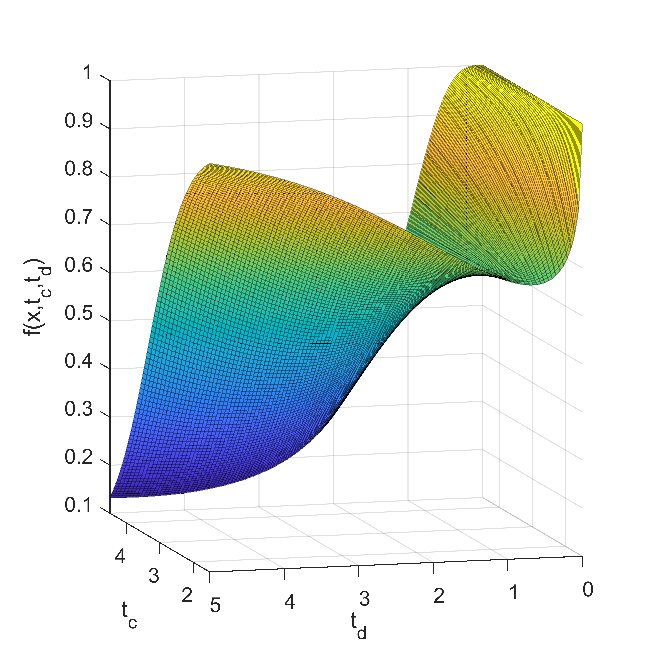
\includegraphics[scale=0.85]{FIG_obj_fn.eps}
	\captionsetup{width=.85\linewidth}
	\caption{Example computer model output over the support of the calibration parameter $t_c$ and the design parameter $t_d$.}
	\label{fig:example_output}
\end{figure}
%
For any value of $x$ and $t_c$, the optimal (minimizing) value of $t_d$ is $(4/3)(t_c-1)$.
%
Suppose that the calibration parameter's ``true'' value is functionally dependent on the design input, with the relationship:
%
\[\theta_c(t_d)= 2.25 - .75 \frac{ \exp\left(40\left(\frac{t_d-1.5}{.75}-.5\right)\right)} {1 + \exp\left( 40\left(\frac{t_d-1.5}{.75}-.5\right) \right)}.\]
%
Figure \ref{fig:SA_relationship} shows this relationship.
%
\begin{figure}
	\centering
	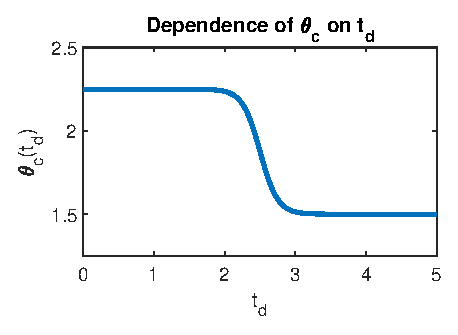
\includegraphics[scale=0.85]{FIG_theta_1_dependence_on_t2}
	\captionsetup{width=.85\linewidth}
	\caption{True value of the calibration parameter $\theta_1$ for each value in the domain of $t_2$}
	\label{fig:SA_relationship}
\end{figure}
%
Figure \ref{fig:true_vals} shows the locations of the true and optimal values (respectively) of $\theta_c$ and $\theta_d$.
%
\begin{figure}
	\centering
	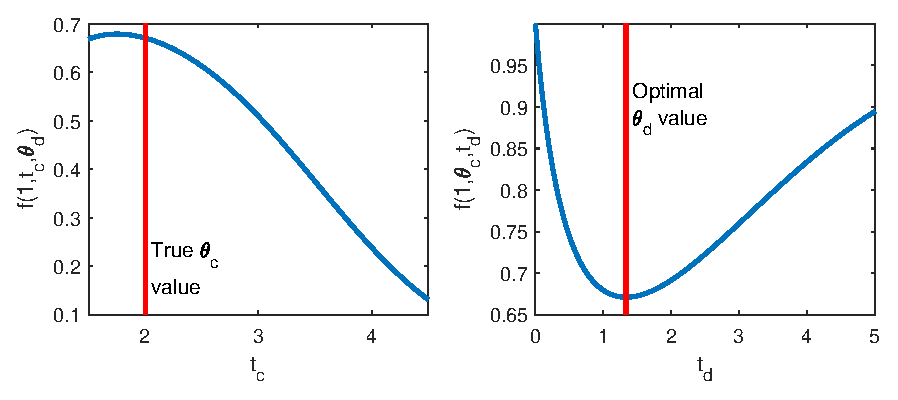
\includegraphics[scale=0.85]{FIG_true_optimal_theta1_theta2.eps}
	\captionsetup{width=.85\linewidth}
	\caption{The top plot shows the computer model output at $x=1$ and optimal design setting for each value of the calibration parameter $t_c$. The bottom plot show the model output at $x=1,t_c=\theta_c(t_d)$ for each value of the design parameter $t_d$.}
	\label{fig:true_vals}
\end{figure}
%
There it is clear that the true value of $\theta_c$ is far from optimal, in the sense that if this value \textit{were} within our control (which, being a calibration parameter, it is not), we would prefer to place it at the upper end of its support, at 4.5.
%
Thus $\eta$ showcases the ability of DCTO to perform simultaneously both calibration and design in the case when our ``truth-seeking'' goals and our design goals are in tension.
%

% 
We apply DCTO to four versions of the problem.
%
First, we assume that $\eta$ is free from discrepancy -- i.e. that $\eta(x,\theta_c,t_d)$ is an unbiased estimator of the ``true'' system $f(x,t_d)$.
%
The other three versions each assume that $\eta$ suffers from some form of discrepancy.
%
Let $f_1,f_2,f_3$ denote the ``true'' systems in these three cases.
%
We set 
%
\begin{align}
	f_1(x,t_d) &= \eta(x,\theta_c,t_d) \left(1-a(x-.5)(x-1)/x) \right)\label{eq:objs1} \\
	f_2(x,t_d)&= \eta(x,\theta_c,t_d) - a(x-.5)(x-1)\left(t_d-\frac43\right)^2 + b\label{eq:objs2}\\
	f_3(x,t_d)&=\eta(x,\theta_c,t_d) + axt_d+b\label{eq:objs3}
\end{align}
%
where $a,b$ are constants which determine how severe the discrepancy is in each case. 
%
The function $f_1$ has a multiplicative discrepancy dependent only on $x$ and $a$. 
%
This discrepancy does not affect the optimal value of $t_d$.  
%
The discrepancies of $f_2$ and $f_3$ are both additive.
%
Figure \ref{fig:discrepancies} shows the discrepancies for two different versions (corresponding to different settings of $(a,b)$) of each $f_i$.
%
\begin{figure*}
	\centering
	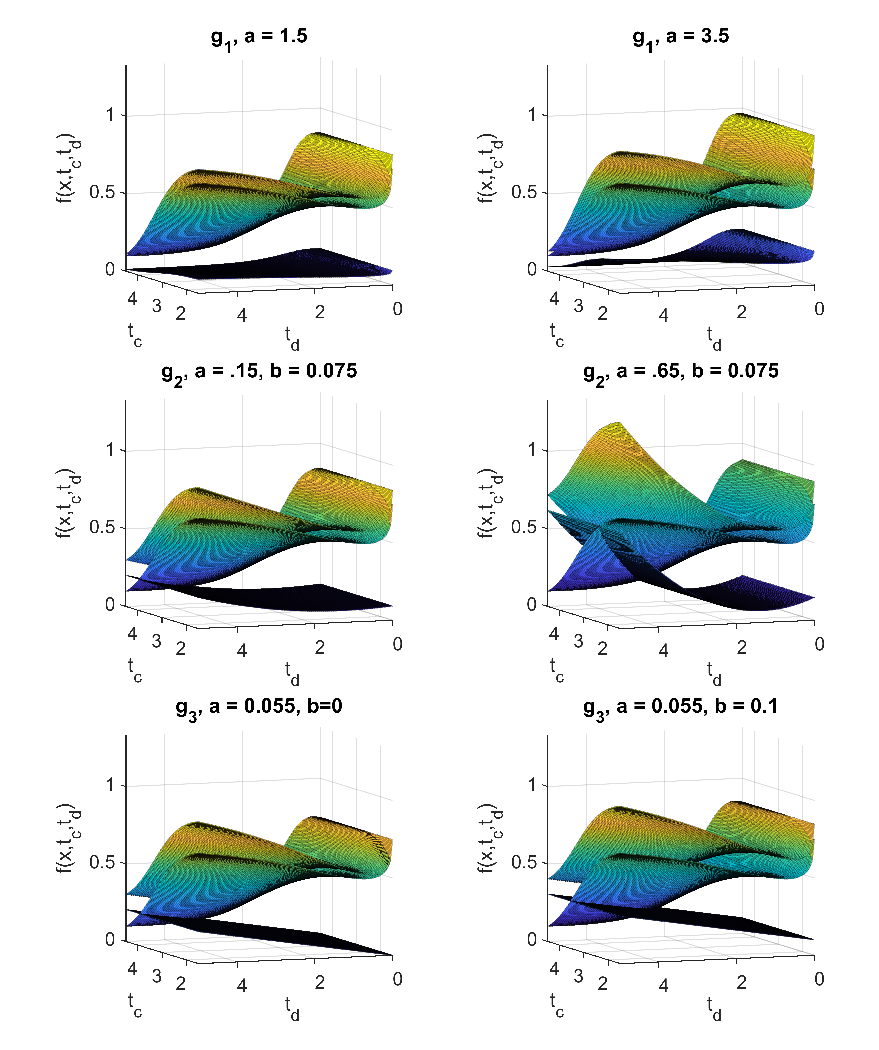
\includegraphics[scale=0.85]{FIG_six_discrepancies.eps}
	\captionsetup{width=.85\linewidth}
	\caption{The $i^{\text{th}}$ row shows $f_i$ (the objective function with discrepancy), $\eta$ (the computer model), and the discrepancy $f_i-\eta$, all at $x=0.75$. In each row, a less aggressive version of the discrepancy appears on the left, and a more aggressive on the right. In each plot, the topmost surface is $f_i$, the middle surface is $\eta$, and the bottom surface is the discrepancy $f_i-\eta$.}
	\label{fig:discrepancies}
\end{figure*}
%

%
We apply DCTO with and without adaptive sampling to each of seven cases, without using an emulator: the non-discrepancy case, and the two different versions of each $f_i$ shown in Figure \ref{fig:discrepancies}.
%
In each case, we gather 30 ``observations'' of $f_i$ on a latin hypercube design over the supports of $x$ and $t_d$, setting $\theta_c$ equal to its ``true'' value of $\theta_c(t_d)$.
%
After standardizing the response to have mean 0 and standard deviation 1, we add i.i.d.\ N(0,0.05) noise to the response.
%
An example of the resulting ``observations'' from non-adaptive DCTO, with noise, appears in Figure \ref{fig:observed_data}.
%
\begin{figure}
	\centering
	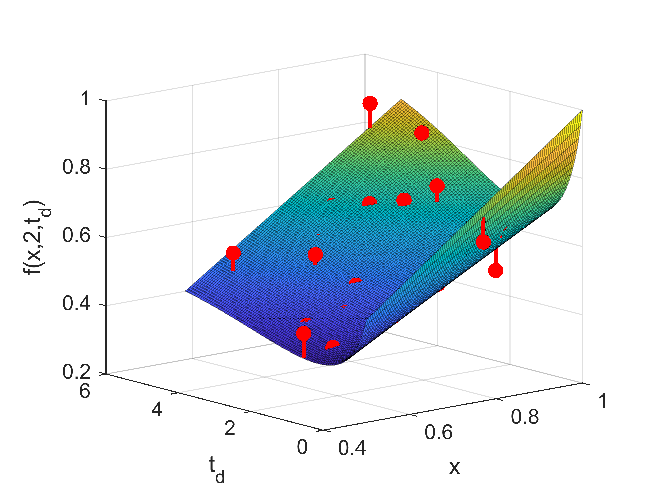
\includegraphics[scale=0.85]{FIG_observed_data}
	\captionsetup{width=.85\linewidth}
	\caption{Noisy observations of the system, and the true system mean, for $f=f_0$ (no discrepancy).}
	\label{fig:observed_data}
\end{figure}
%
We carry out DCTO using Metropolis-Hastings-within-Gibbs MCMC, drawing 8000 realizations each (discarding the first 4000 as burn-in) of $t_c,t_d,\boldsymbol\rho_{\delta},\lambda_{\delta},\sigma^2_d$, where $\boldsymbol\phi_\delta = (\boldsymbol\rho_\delta^T,\lambda_\delta)^T$.
%
For the adaptive sampling application of DCTO, we begin the MCMC with 0 observations of $f_i$, making a new observation after every 100 steps of MCMC until we reached the total budget of 20.
%
An example of the resulting difference between the adaptive sampling approach and relying on a space filling design, with regard to the sampling distribution of our observations of the objective function, appears in Figure \ref{fig:AS_distribution}.
%
\begin{figure}
	\centering
	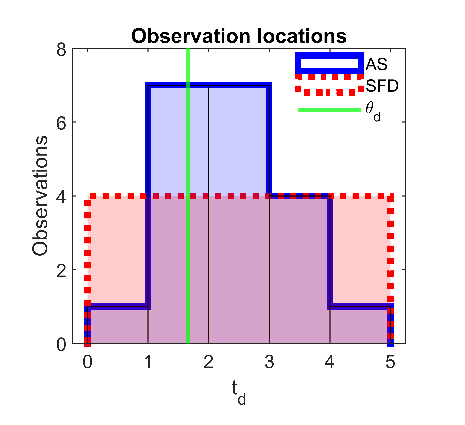
\includegraphics[scale=0.85]{FIG_AS_vs_SFD_obs_locs}
	\captionsetup{width=.85\linewidth}
	\caption{Design input values for observations made under the adaptive sampling approach (AS) and under a space-filling design (SFD), along with the optimal value $\theta_d$ of the design input.}
	\label{fig:AS_distribution}
\end{figure}
%
There, one can see that the adaptive sampling approach manages to expend its budget on observations that are near to the region of design interest.
%
This explains the superior performance of adaptive sampling (discussed below) in both design and in calibration (since the value of the calibration parameter is dependent upon that of the design input).
%
This ameliorative effect would likely be even greater in a higher-dimensional case, in which a space-filling design would (due to the curse of dimensionality) tend to generate observations even farther from the region of design interest.
%

%
In both versions of DCTO, we modularize the analysis by drawing each of $\boldsymbol\theta_c,\boldsymbol\rho_\delta,\lambda_\delta$ using the likelihood based only on $(\mathbf y_s^T,\mathbf y_r^T)^T$ rather than on $(\mathbf y_s^T,\mathbf y_r^T,\mathbf y_t^T)^T$.
%
Convergence was verified visually and by the Gelman-Rubin statistic ($\approx 1.01$; \cite{Gelman1992a}, \cite{Gelman1992a}).
%

%
The resulting optimal design settings and calibration parameter value at the optimum vary in the discrepancy cases, though $\theta_c(\theta_d)$ is near 2.16 in each case.
%
Representative results from performing DCTO with adaptive sampling in each discrepancy case appear in Figure \ref{fig:sdoe_vs_pdoe}, along with results from applying DCTO non-adaptively (using a space-filling set of observations).
%
A summary of the results of thirty applications of DCTO both with and without adaptive sampling, for each of the discrepancy cases, appears in Table \ref{table:vars_and_rmses}.
%
\begin{figure*}
	\centering
	\begin{tabular}{p{.13\linewidth} c c}
	$f_0$ (no discrepancy) &
	\raisebox{-.5\height}{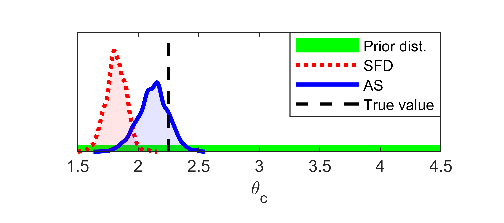
\includegraphics[scale=0.85]{FIG_dual_calib_SDOE_comp_theta1-d0}} &
	\raisebox{-.5\height}{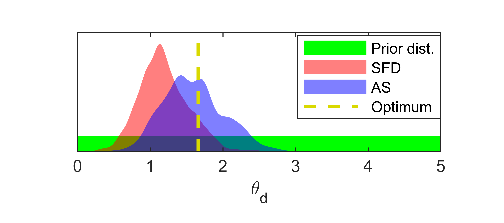
\includegraphics[scale=0.85]{FIG_dual_calib_SDOE_comp_theta2-d0}}\\
	$f_1,\ a=1.5$ & 
	\raisebox{-.5\height}{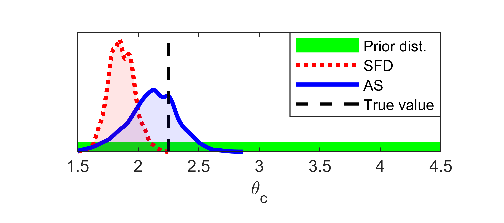
\includegraphics[scale=0.85]{FIG_dual_calib_SDOE_comp_theta1-d1}} &
	\raisebox{-.5\height}{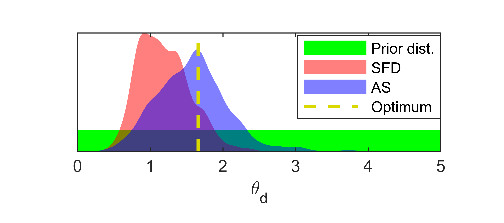
\includegraphics[scale=0.85]{FIG_dual_calib_SDOE_comp_theta2-d1}}\\
	$f_1,\ a=3.5$ & 
	\raisebox{-.5\height}{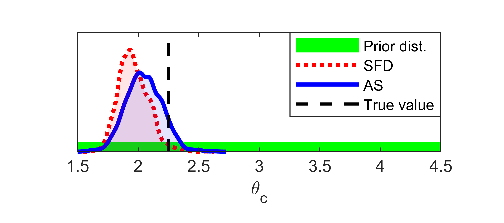
\includegraphics[scale=0.85]{FIG_dual_calib_SDOE_comp_theta1-d2}} &
	\raisebox{-.5\height}{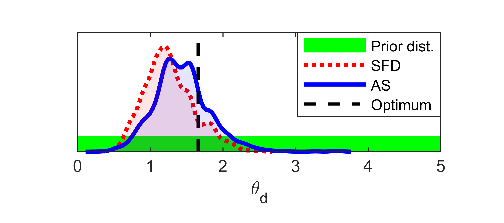
\includegraphics[scale=0.85]{FIG_dual_calib_SDOE_comp_theta2-d2}}\\
	$f_2$, $a=.15$, $b=.075$ &
	\raisebox{-.5\height}{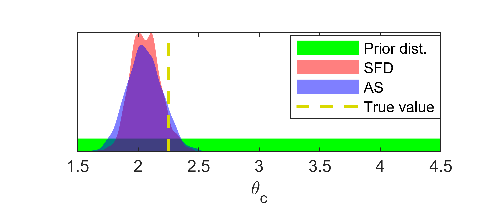
\includegraphics[scale=0.85]{FIG_dual_calib_SDOE_comp_theta1-d3}} &
	\raisebox{-.5\height}{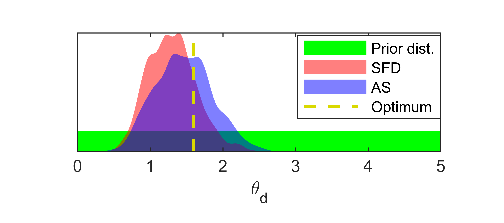
\includegraphics[scale=0.85]{FIG_dual_calib_SDOE_comp_theta2-d3}}\\
	$f_2$, $a=.65$, $b=.075$ &
	\raisebox{-.5\height}{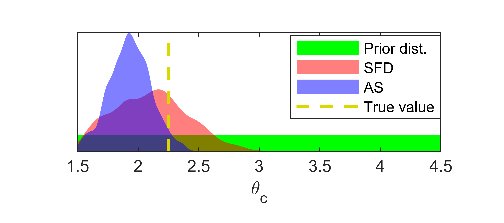
\includegraphics[scale=0.85]{FIG_dual_calib_SDOE_comp_theta1-d4}} &
	\raisebox{-.5\height}{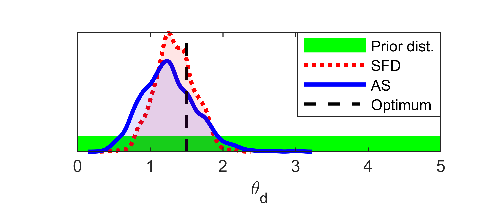
\includegraphics[scale=0.85]{FIG_dual_calib_SDOE_comp_theta2-d4}}\\
	$f_3$, $a=.055$, $b=0$ &
	\raisebox{-.5\height}{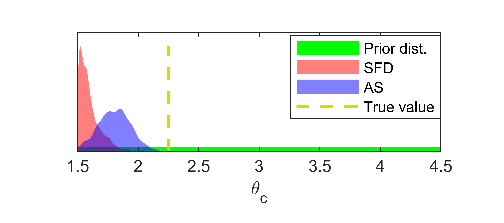
\includegraphics[scale=0.85]{FIG_dual_calib_SDOE_comp_theta1-d5}} &
	\raisebox{-.5\height}{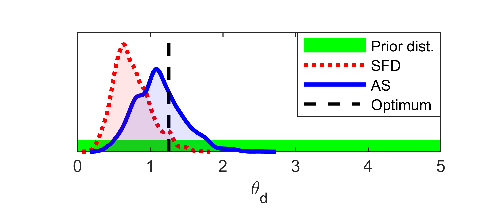
\includegraphics[scale=0.85]{FIG_dual_calib_SDOE_comp_theta2-d5}}\\
	$f_3$, $a=.055$, $b=.1$ &
	\raisebox{-.5\height}{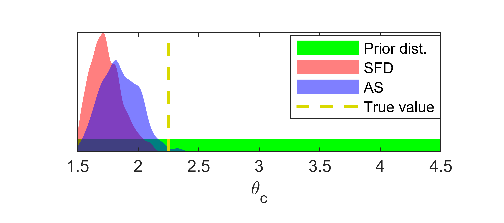
\includegraphics[scale=0.85]{FIG_dual_calib_SDOE_comp_theta1-d6}} &
	\raisebox{-.5\height}{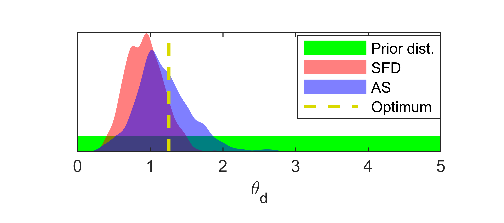
\includegraphics[scale=0.85]{FIG_dual_calib_SDOE_comp_theta2-d6}}
	\end{tabular}
	\captionsetup{width=.85\linewidth}
	\caption{Prior and posterior distributions of the calibration parameter $\theta_c$ and design parameter $\theta_d$, along with their true/optimal values, for DCTO with adaptive sampling (AS) and with predetermined space-filling design (SFD) in each of the cases studied. For each $f_i$, $a$ and $b$ control the size of the discrepancy as specified in Equations (\ref{eq:objs1},\ref{eq:objs2},\ref{eq:objs3}).}
	\label{fig:sdoe_vs_pdoe}
\end{figure*}
%
\begin{table}[]
	\centering
	\begin{tabular}{l|cc|cc}
		&\multicolumn{2}{c|}{$\widehat\theta_c$ RMSE}&
		\multicolumn{2}{c}{$\widehat\theta_d$ RMSE} \\ \hline
		Objective    & AS   & SFD & AS    & SFD   \\ \hline
		$f_0$ (no discrepancy)             & 0.188 & 0.433 & 0.163 & 0.479\\ \hline
		$f_1,\ a=1.5$       & 0.233 & 0.32 & 0.243 & 0.414\\ \hline
		$f_1,\ a=3.5$       & 0.188 & 0.247 & 0.213 & 0.393\\ \hline
		$f_2$, $a=.15$, $b=.075$       & 0.221 & 0.263 & 0.187 & 0.348\\ \hline
		$f_2$, $a=.65$, $b=.075$       & 0.228 & 0.16 & 0.183 & 0.206\\ \hline
		$f_3$, $a=.055$, $b=0$       & 0.452 & 0.506 & 0.182 & 0.329\\ \hline
		$f_3$, $a=.055$, $b=.1$       & 0.448 & 0.468 & 0.167 & 0.292\\ \hline
	\end{tabular}
	\caption{Posterior root mean square error (RMSE) for the calibration variable $\theta_c$ and the design variable $\theta_d$, for DCTO with adaptive sampling (AS) and a predetermined space-filling design (SFD). The estimator $\widehat{\theta_i}$ is the posterior mean of $t_i$ for $i=c,d$. For each $f_i$, $a$ and $b$ control the size of the discrepancy as specified in Equations (\ref{eq:objs1},\ref{eq:objs2},\ref{eq:objs3}).} 
	\label{table:vars_and_rmses}
\end{table}
%

%
The results show superior performance for the adaptive sampling DCTO over DCTO using a space-filling design of experiments for the true phenomenon (or high-fidelity model, in a case of calibrating a low-fidelity model to use for design purposes).
%
The adaptive DCTO posterior means have lower RMSEs in all cases for $\theta_d$, and in all cases except one for $\theta_c$.
%
This demonstrates a useful robustness of adaptive DCTO to model misspecification, specifically in the case that the model treats as constant a calibration parameter that is more properly understood as functionally dependent upon other model inputs.
%
By using the CTO-driven estimate $\widehat\theta_d$ to sample from the region of interest, DCTO learns from observations such that $\theta_c(\widehat\theta_d)$ is near to the value $\theta_c(\theta_d)$.
%
This promotes better calibration with respect to the region of interest, and thereby better estimation of the optimal design settings.
%
By relying on DCTO rather than on performing KOH using samples gathered using heuristic optimization methods, or other RSM approaches, we achieve these estimates with quantification of all relevant model-driven uncertainty with respect to the values of $\theta_c$ and $\theta_d$.
%

%
\section{Application: Dynamic vibration system}\label{sec:dvs}
%
The dynamic vibration system (DVS) to which we apply DCTO is shown in Figure \ref{fig:dvs}.
%
\begin{figure}
	\centering
	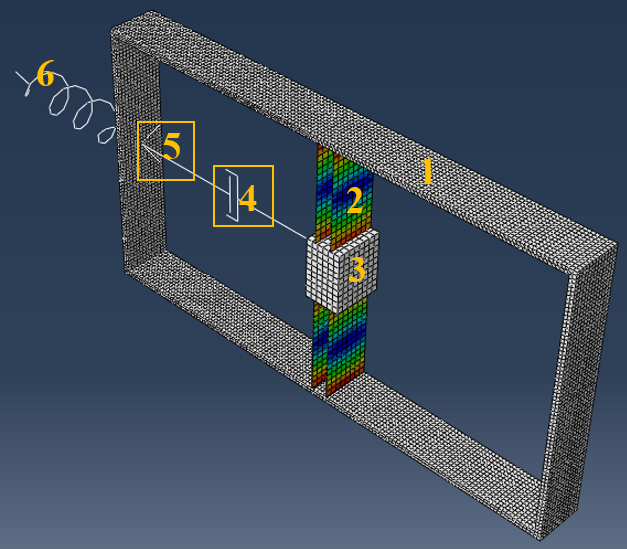
\includegraphics[width=2in]{FIG_dvs_illustration}
	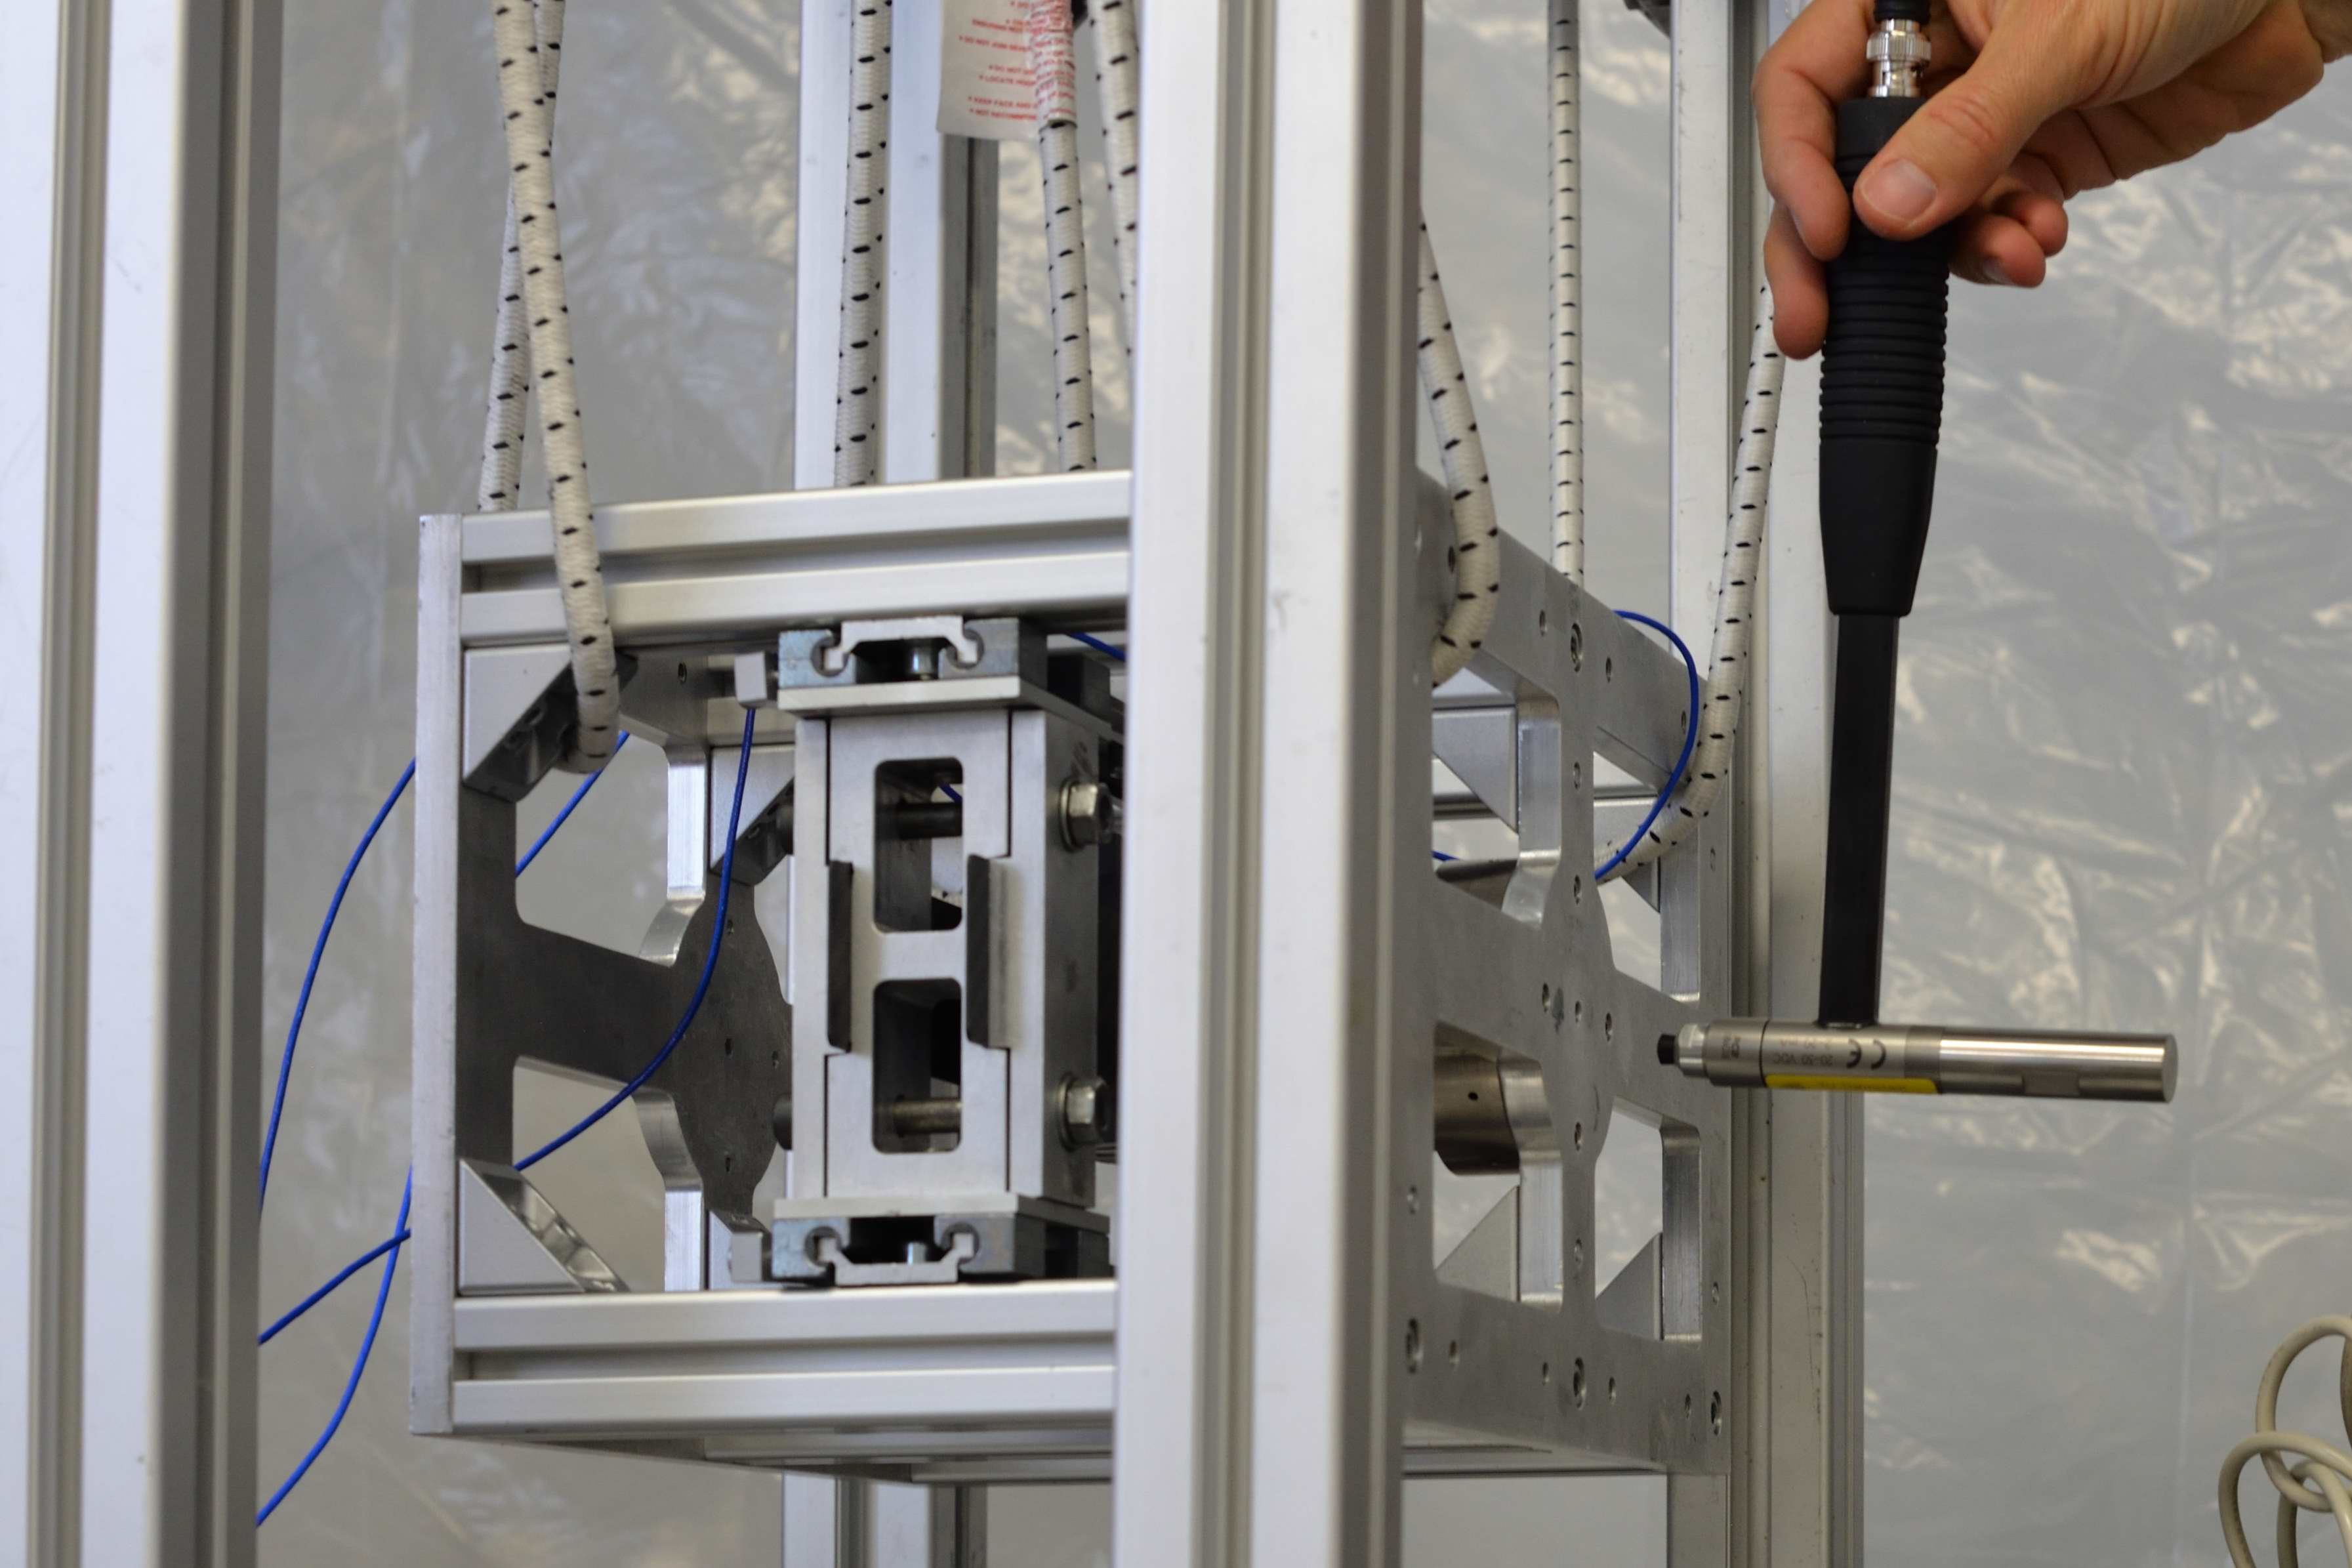
\includegraphics[width=2in]{DSC_5206_crop}
	\captionsetup{width=.85\linewidth}
	\caption{The dynamic vibration system, schematic and photograph. (1) The frame, (2) the beam, (3) the mass oscillator, (4) the spring, (5) the damper, and (6) the gain.}
	\label{fig:dvs}
\end{figure}
%
In the DVS, an impulse force is applied to the frame of the system, causing the frame and the mass oscillator to accelerate.
%
From the resulting acceleration over time of the mass oscillator, we can calculate the damping ratio $\zeta$ of the system as
\[
\psi = \frac1n \log\frac{x(t)}{x(t+nT)},\quad \zeta = \frac1{\sqrt{1+\left(\frac{2\pi}{\psi}\right)^2}}
\]
%
where $t$ is the time in seconds of the first peak value of mass acceleration, $T$ is the time period of one oscillation, and $n$ is the total number of time steps -- i.e. the number of periods of the oscillation -- used in the calculation.
%
We use a finite element (FE) model of the system in conjunction with a set of 12 experimental observations in order to calibrate the elastic modulus of the spring.
%
For the simulation data, $n=1$, whereas for the experimental data we use $n=4$ in order to account for measurement error TODO VERIFY THIS EXPLANATION.
%
Due to the high computational cost of the FE model (roughly TODO HOW MANY seconds per model evaluation), we rely on a set of 98 runs for the calibration.
%
In addition to the calibration, we undertake simultaneous design using these model runs and experimental observations in order to minimize the damping ratio of the system by tuning the value of the gain.
%

%
Thus in our application, the inputs of the FE system are the mass $m$ of the oscillator (in kilograms), the elastic modulus $k$ of the spring (in Newtons per meter), and the gain $g$ (in Newtons per meter per second).
%
The relevant output of the system is the damping ratio.
%
The simulator is implemented in the commercial finite element software ABAQUS \cite{Abaqus2012}.
%
The experimental design for the simulator runs is a latin hypercube over a range of the inputs that covers those of the available experimental data for the known inputs $m$ and $g$, and that covers a plausible range of values for the calibration input $k$.
%
The experimental design is a full factorial design over three different mass levels (0.7853, 0.9653, and 1.1493kg) and four different gain levels (0, 8, 41, and 95 Ns/m).
%
The expected elastic modulus for the system is 6.2e+10, as estimated by the leaf spring manufacturer.
%

%
Since our goal is to minimize the damping ratio, we set our target outcomes $y_t$ to be 0 across a range of oscillator masses.
%
Specifically, we set a grid of size 8 over the range of oscillator masses present in the simulation and experimental data, with target outcome 0 for each point in that grid.
%
We define our prior GP surrogate for the FE model using a mean function found via degree-2 polynomial regression on the available FE runs.
%
For the hyperparameters of the surrogate's covariance function, we estimate them as MLEs using the quasi-Newton BFGS method \cite{Fletcher2013}.
%
We perform 10,000 iterations of MCMC using this surrogate and set of target observations, of which the first half are discarded as burn-in.
%
The convergence of the resulting MCMC chains is assessed both visually and using the Gelman-Rubin statistic ($\approx1.01$ and $1.001$ for calibration and design respectively), \cite{Gelman1992a}).
%

%
The total wall time required for the MCMC to complete DCTO in this case was 94 seconds (on a laptop with an Intel Core i7-9750H CPU and 16GB of RAM).
%
The posterior distributions of the calibration and design inputs are are shown in Figure \ref{fig:dvs_calib_and_design}.
%
\begin{figure}
	\centering
	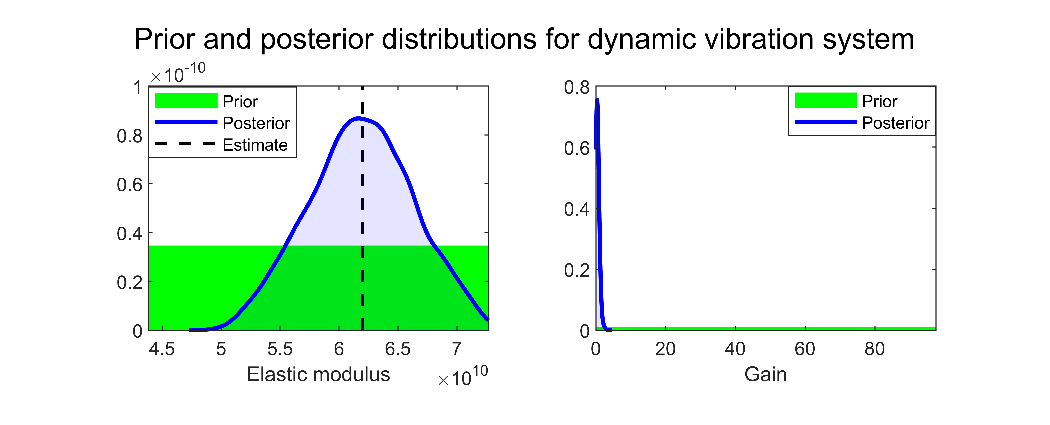
\includegraphics[scale=0.85]{FIG_DVS_DCTO_input_posteriors}
	\captionsetup{width=.85\linewidth}
	\caption{The posterior distributions of the calibration and design inputs, respectively, along with their (uniform) priors. The very narrow posterior distribution of gain is concentrated at the minimum of its support.}
	\label{fig:dvs_calib_and_design}
\end{figure}
%
Strong Bayesian learning has occurred, particularly for the design input.
%
The posterior distribution of the elastic modulus for the system assigns high likelihood to the expected value of 6.2e10, with a posterior mean of 6.188e10.
%
For comparison with our design results, we also apply the NSGA-II algorithm \cite{Deb2002}, a gradient-free genetic algorithm, to the trained GP model surrogate.
%
We use 100 generations and a population size 50, taking a total of 48 seconds of computation (wall time).
%
Whereas our method performs both calibration and design, NSGA-II cannot be used for calibration, and so we apply it to a model calibrated with a point estimate (the posterior mean) of elastic modulus from our method's results.
%
The results of NSGA-II agree with our own, in finding the optimal gain setting to be 0.
%

%
We also use the surrogate model to estimate also the posterior predictive distribution of the system after DCTO.
%
Figure \ref{fig:dvs_output} shows the resulting posterior distributions of model output at various levels of oscillator mass, along with the distributions of both experimental and simulator system output.
%
\begin{figure}
	\centering
	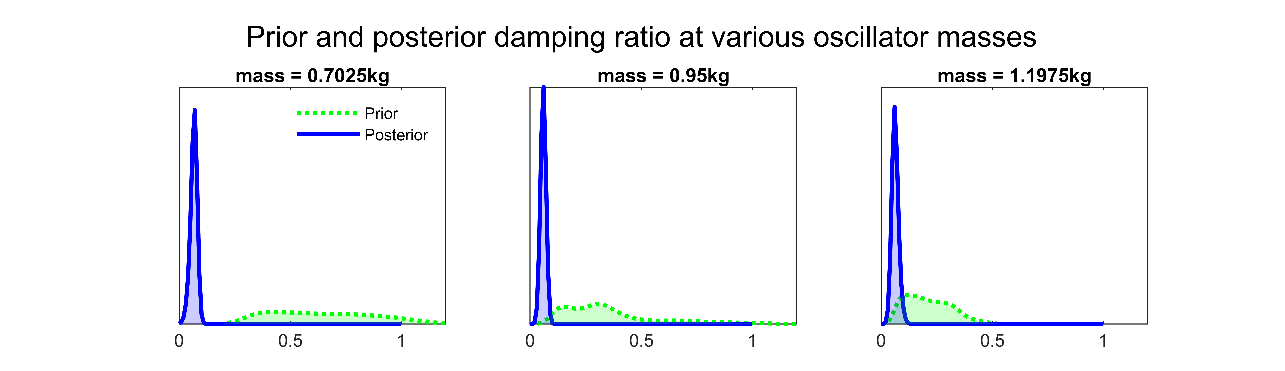
\includegraphics[scale=0.85]{FIG_DVS_DCTO_prior_and_posterior_output}
	\captionsetup{width=.85\linewidth}
	\caption{The posterior distributions of the model output at three different levels of the operational domain, along with their prior distributions. The posteriors constitute a notable performance increase over the priors.}
	\label{fig:dvs_output}
\end{figure}
%
For comparison, the figure also includes the output of the surrogate model using the posterior mean of elastic modulus along with the NSGA-II estimate of optimal gain.
%
Note that the predicted model outputs fall at the bottom of the ranges of observed model outputs across the domain of oscillator masses, implying a successful design outcome for the system has been achieved.
%

%
\section{Conclusion}\label{sec:conclusion}
%
DCTO provides a method for generalizing the KOH framework for model calibration to include design.
%
The result secures the benefits of KOH both for calibration and for design.
%
This includes the ability to quantify uncertainty remaining in the true value of the calibration parameter, the optimal settings for the design input, and the resulting model output.
%
DCTO provides a computationally efficient method of propagating the uncertainties remaining from KOH calibration through the design procedure.
%
In the case when observations of the real system can be carried out sequentially at adaptively chosen locations, DCTO is robust to model misspecification where the calibration parameter is functionally dependent on the value of the design input and the model fails to reflect this.
%
In such a case, if the functional form of the dependence of $\boldsymbol\theta_c$ on $\boldsymbol\theta_d$ is of interest, then state-aware calibration should be used.
%
However, if one only wishes to estimate the calibration parameter at the optimal design settings, then DCTO provides a means of doing so.
%
In this application, DCTO with adaptive sampling uses information from both the sequentially-performed observations of the real system and from the existing computer model to identify new sampling locations.
%
Future work on this subject will include pairing adaptive sampling DCTO with other methodologies for selecting new sampling locations, such as EGO and SUR.
%

\bigskip

%\begin{center}
%{\large\bf SUPPLEMENTARY MATERIAL}
%\end{center}
%
%\begin{description}
%
%\item[Title:] Brief description. (file type)
%
%\item[R-package for  MYNEW routine:] R-package �MYNEW� containing code to perform the diagnostic methods described in the article. The package also contains all datasets used as examples in the article. (GNU zipped tar file)
%%
%\item[HIV data set:] Data set used in the illustration of MYNEW method in Section~ 3.2. (.txt file)
%
%\end{description}

\bibliographystyle{asmems4}

\bibliography{lit_review}
%
%\section*{Appendix: Validation of DCTO}
%
%%
%In order to validate the performance of simultaneous calibration and design under DCTO against a two-step calibration and design approach, we use the system described by Equations (\ref{eq:objs1},\ref{eq:objs2},\ref{eq:objs3}) where the value of calibration parameter does not depend on the value of the design input. 
%%
%We employ a space-filling design of observations of the ``true'' system under both approaches. 
%%
%For the two-step approach, we carry apply traditional KOH calibration of $\theta_c$, followed by a second step using the KOH framework for design, obtaining a distribution of $\theta_d$. 
%%
%The first step is thus essentially DCTO with $\mathbf{x_t},\mathbf{y_t}$ as empty (null) vectors, and the second step uses the distributions obtained in the first step to estimate $\theta_d$.
%%
%Thus, the comparison between the unified approach, i.e. DCTO, and the two-step calibration and design approach shows the difference between DCTO and performing design on a system which has been calibrated using traditional methods and serves as validation of the former.
%%
%
%%
%Figure \ref{fig:no_discrep_results} shows the results of DCTO and two-step calibration and design for $f_0$, the case of no discrepancy.
%%
%\begin{figure}
%	\centering
%	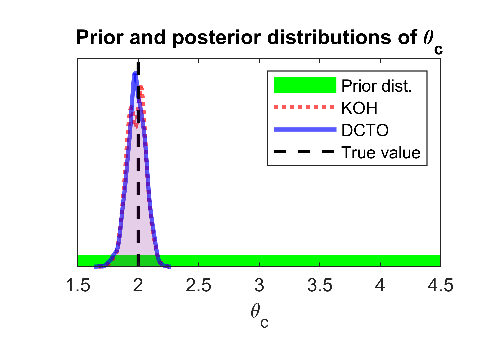
\includegraphics[scale=0.85]{FIG_dual_calib_post_theta1-d0}
%	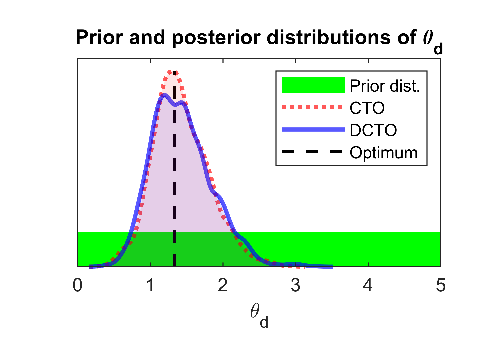
\includegraphics[scale=0.85]{FIG_dual_calib_post_theta2-d0}
%	\captionsetup{width=.85\linewidth}
%	\caption{Prior and posterior distributions of the calibration parameter $\theta_c$ and design parameter $\theta_d$, along with their true/optimal values, for DCTO and two-step calibration and design carried out when there is no discrepancy between the true system described by Equation (\ref{eq:f0}) (the case of no discrepancy) and the computer model.}
%	\label{fig:no_discrep_results}
%\end{figure}
%%
%The two methods deliver comparable results, illustrating that extending calibration to include design does not undermine the performance of either task.
%%
%Strong Bayesian learning has occurred for both parameters, in that the posterior distributions of $\theta_c,\theta_d$ are peaked around their true and optimal values, respectively.
%%
%KOH gives a similar posterior for $\theta_c$, showing that the expansion of DCTO to undertake design has not interfered with its calibration performance.
%%
%The skew apparent in the posterior distributions of $\theta_d$ occur in all of the results gathered here, and is likely due to the shape of the objective function $f$, which is much more informative below $\theta_d$ than above it in that it increases sharply for $t_d<\theta_d$ and increases much more gently for $t_d>\theta_d$.
%%
%
%%
%We performed each procedure 30 times on each of the seven different discrepancy situations (no discrepancy, and a large and small version of each of three discrepancies).
%%
%The results are summarized in Table \ref{table:val_vars_and_rmses}.
%%
%\begin{table*}[]
%	\centering
%	\begin{tabular}{l|cc|cc}
%		&\multicolumn{2}{c|}{Posterior $\theta_c$ var.}&
%		\multicolumn{2}{c}{Posterior $\theta_d$ var.} \\ \hline
%		Discrepancy    & DCTO   & KOH+design & DCTO    & KOH+design   \\ \hline
%		$f_0$ (no discrepancy)              & 0.00633 & 0.00619 & 0.145 & 0.129\\ \hline
%		$f_1$, $a=1.5$       & 0.0140 & 0.0137 & 0.149 & 0.129\\ \hline
%		$f_1$, $a=3.5$       & 0.0141 & 0.0140 & 0.149 & 0.131\\ \hline
%		$f_2$, $a=.15$, $b=.075$       & 0.0143 & 0.0141 & 0.135 & 0.116\\ \hline
%		$f_2$, $a=.65$, $b=.075$       & 0.0609 & 0.0608 & 0.0804 & 0.0731\\ \hline
%		$f_3$, $a=.055$, $b=0$       & 0.0134 & 0.0135 & 0.0882 & 0.0743\\ \hline
%		$f_3$, $a=.055$, $b=.1$       & 0.0143 & 0.0142 & 0.0945 & 0.0814\\ \hline
%	\end{tabular}\\
%	\vspace{.25in}
%	\begin{tabular}{l|cc|cc}
%		&\multicolumn{2}{c|}{$\widehat\theta_c$ RMSE}&
%		\multicolumn{2}{c}{$\widehat\theta_d$ RMSE} \\ \hline
%		Discrepancy    & DCTO   & KOH+CTO & DCTO    & KOH+CTO   \\ \hline
%		$f_0$ (no discrepancy)              & 0.0790 & 0.0795 & 0.120 & 0.121\\ \hline
%		$f_1$, $a=1.5$       & 0.0955 & 0.0956 & 0.149 & 0.144\\ \hline
%		$f_1$, $a=3.5$       & 0.137 & 0.139 & 0.209 & 0.209\\ \hline
%		$f_2$, $a=.15$, $b=.075$       & 0.109 & 0.106 & 0.130 & 0.127\\ \hline
%		$f_2$, $a=.65$, $b=.075$       & 0.158 & 0.155 & 0.123 & 0.121\\ \hline
%		$f_3$, $a=.055$, $b=0$       & 0.294 & 0.292 & 0.0919 & 0.0919\\ \hline
%		$f_3$, $a=.055$, $b=.1$       & 0.279 & 0.281 & 0.0995 & 0.0990\\ \hline
%	\end{tabular}
%	\caption{Posterior variance and root mean square error (RMSE) for the calibration variable $\theta_c$ and the design variable $\theta_d$ under both DCTO and two-step calibration and design (KOH+design). The estimator $\widehat{\theta_i}$ is the posterior mean of $t_i$ for $i=c,d$. For each $f_i$, $a$ and $b$ control the size of the discrepancy as specified in Equations (\ref{eq:objs1},\ref{eq:objs2},\ref{eq:objs3}).} 
%	\label{table:val_vars_and_rmses}
%\end{table*}
%%
%The upper table gives the sample mean, over the thirty runs, of the marginal posterior variance of each of $\theta_c$ and $\theta_d$.
%%
%The two procedures generate extremely similar outcomes with respect to $\theta_c$.
%%
%However, the posterior variance for $\theta_d$ under DCTO is slightly higher than that under two-step calibration and design in each of the seven cases considered.
%%
%This is due to the fact that DCTO includes remaining uncertainty about the values of the hyperparameters of the discrepancy GP $\delta(\cdot)$.
%%
%By contrast, design after calibration uses point estimates of those hyperparameters and thus achieves narrower posterior distributions due to excluding this source of uncertainty.
%%
%The lower table gives the root mean square errors (RMSEs) for the posterior means of $\theta_c$ and $\theta_d$, using their true value of 2 for $\theta_c$ and optimal value $4/3$ for $\theta_d$ in discrepancy cases $0,1,2$ and optimal value $1$ for discrepancy 3.
%%
%Again we see very similar outcomes in the two procedures for both parameters.
%%
%In all cases but one, DCTO has slightly higher RMSE for $\theta_d$ than does design after KOH calibration.
%%
%This is to be expected given the above-mentioned wider posterior distributions of $\theta_d$ under DCTO.
%%
%In general, we see that the DCTO expansion of the KOH framework achieves the expected similar results to KOH calibration followed by a design step, though with wider posterior distributions of the design input, because the DCTO approach properly includes in the design step a source of uncertainty (hyperparameters of hte discrepancy GP $\delta(\cdot)$) ignored by the traditional two-step approach.
%%

\end{document}


